This appendix presents the principal components eigenvectors from the Principal Component Analysis (PCA) in section \ref{chap3-data}. Table \ref{chap3-tab:pca-v5-BCS70} presents the eigenvectors for the BCS70 cohort, while table \ref{chap3-tab:pca-v5-NCDS58} displays those for the NCDS58 cohort.

\begin{table}[!hb]
    \centering
    \caption{Principal components eigenvectors for the BCS70 cohort}
    \label{chap3-tab:pca-v5-BCS70}
    \begin{threeparttable}
        
\begin{tabular}{lrrrrr}
\toprule
  & \multicolumn{1}{c}{PC1} & \multicolumn{1}{c}{PC2} & \multicolumn{1}{c}{PC3} & \multicolumn{1}{c}{PC4} & \multicolumn{1}{c}{PC5}\\
\midrule
\addlinespace[0.3em]
\multicolumn{6}{l}{\textbf{Age 26}}\\
\hline
\hspace{1em}Authority & 0.622 & 0.011 & 0.136 & -0.146 & -0.757\\
\hspace{1em}Inequality Aversion & -0.182 & 0.686 & -0.533 & 0.348 & -0.303\\
\hspace{1em}Morale & 0.521 & 0.244 & -0.453 & -0.513 & 0.449\\
\hspace{1em}Political Cynicism & 0.149 & 0.656 & 0.695 & 0.065 & 0.245\\
\hspace{1em}Work Ethic & 0.535 & -0.200 & -0.093 & 0.769 & 0.272\\
\midrule
\hspace{1em}Standard deviation & 1.262 & 1.087 & 0.929 & 0.866 & 0.783\\
\hspace{1em}Proportion of Variance & 0.319 & 0.236 & 0.173 & 0.150 & 0.123\\
\hspace{1em}Cumulative Proportion & 0.319 & 0.555 & 0.727 & 0.877 & 1.000\\
\addlinespace[0.3em]
\multicolumn{6}{l}{\textbf{Age 30}}\\
\hline
\hspace{1em}Authority & 0.614 & -0.162 & -0.050 & 0.281 & -0.718\\
\hspace{1em}Inequality Aversion & 0.153 & 0.702 & 0.013 & -0.638 & -0.278\\
\hspace{1em}Morale & 0.534 & -0.109 & -0.678 & -0.202 & 0.450\\
\hspace{1em}Political Cynicism & 0.326 & 0.605 & 0.221 & 0.592 & 0.359\\
\hspace{1em}Work Ethic & 0.456 & -0.321 & 0.699 & -0.351 & 0.276\\
\midrule
\hspace{1em}Standard deviation & 1.243 & 1.137 & 0.918 & 0.827 & 0.797\\
\hspace{1em}Proportion of Variance & 0.309 & 0.259 & 0.169 & 0.137 & 0.127\\
\hspace{1em}Cumulative Proportion & 0.309 & 0.568 & 0.736 & 0.873 & 1.000\\
\addlinespace[0.3em]
\multicolumn{6}{l}{\textbf{Age 42}}\\
\hline
\hspace{1em}Authority & 0.570 & -0.360 & -0.004 & -0.519 & -0.526\\
\hspace{1em}Inequality Aversion & 0.172 & 0.722 & 0.172 & 0.280 & -0.584\\
\hspace{1em}Morale & 0.462 & -0.048 & -0.749 & 0.466 & 0.079\\
\hspace{1em}Political Cynicism & 0.517 & 0.474 & 0.122 & -0.368 & 0.598\\
\hspace{1em}Work Ethic & 0.406 & -0.350 & 0.628 & 0.548 & 0.135\\
\midrule
\hspace{1em}Standard deviation & 1.184 & 1.124 & 0.968 & 0.882 & 0.787\\
\hspace{1em}Proportion of Variance & 0.281 & 0.253 & 0.187 & 0.156 & 0.124\\
\hspace{1em}Cumulative Proportion & 0.281 & 0.533 & 0.721 & 0.876 & 1.000\\
\bottomrule
\end{tabular}

        % \begin{tablenotes}[flushleft]
        %     \footnotesize{\item \textit{Notes}: Signs of the eigenvectors have been inverted for age 30 and age 42 in order to have the same axis direction for the first principal component. The attitude toward Inequality Aversion (IA) is removed for the PCA on the BCS70 cohort at the age of 26 years because only one statement is available.}
        % \end{tablenotes}
    \end{threeparttable}
\end{table}

\begin{table}[!htb]
    \centering
    \caption{Principal components eigenvectors for the NCDS58 cohort}
    \label{chap3-tab:pca-v5-NCDS58}
    \begin{threeparttable}
        
\begin{tabular}{lrrrrr}
\toprule
  & \multicolumn{1}{c}{PC1} & \multicolumn{1}{c}{PC2} & \multicolumn{1}{c}{PC3} & \multicolumn{1}{c}{PC4} & \multicolumn{1}{c}{PC5}\\
\midrule
\addlinespace[0.3em]
\multicolumn{6}{l}{\textbf{Age 33}}\\
\hline
\hspace{1em}Authority & 0.607 & -0.150 & 0.155 & -0.546 & 0.535\\
\hspace{1em}Inequality Aversion & 0.006 & 0.730 & -0.072 & 0.353 & 0.580\\
\hspace{1em}Morale & 0.548 & -0.077 & 0.551 & 0.591 & -0.201\\
\hspace{1em}Political Cynicism & 0.276 & 0.654 & 0.053 & -0.414 & -0.567\\
\hspace{1em}Work Ethic & 0.504 & -0.102 & -0.815 & 0.237 & -0.122\\
\midrule
\hspace{1em}Standard deviation & 1.250 & 1.162 & 0.901 & 0.851 & 0.741\\
\hspace{1em}Proportion of Variance & 0.313 & 0.270 & 0.162 & 0.145 & 0.110\\
\hspace{1em}Cumulative Proportion & 0.313 & 0.583 & 0.745 & 0.890 & 1.000\\
\addlinespace[0.3em]
\multicolumn{6}{l}{\textbf{Age 42}}\\
\hline
\hspace{1em}Authority & 0.605 & -0.141 & -0.156 & 0.369 & 0.674\\
\hspace{1em}Inequality Aversion & 0.173 & 0.713 & 0.178 & -0.559 & 0.342\\
\hspace{1em}Morale & 0.500 & -0.245 & -0.542 & -0.534 & -0.333\\
\hspace{1em}Political Cynicism & 0.446 & 0.521 & 0.038 & 0.480 & -0.546\\
\hspace{1em}Work Ethic & 0.395 & -0.375 & 0.805 & -0.187 & -0.144\\
\midrule
\hspace{1em}Standard deviation & 1.258 & 1.101 & 0.916 & 0.875 & 0.775\\
\hspace{1em}Proportion of Variance & 0.317 & 0.242 & 0.168 & 0.153 & 0.120\\
\hspace{1em}Cumulative Proportion & 0.317 & 0.559 & 0.727 & 0.880 & 1.000\\
\addlinespace[0.3em]
\multicolumn{6}{l}{\textbf{Age 50}}\\
\hline
\hspace{1em}Authority & 0.531 & -0.134 & 0.063 & -0.816 & -0.173\\
\hspace{1em}Inequality Aversion & 0.554 & 0.296 & -0.075 & 0.441 & -0.637\\
\hspace{1em}Morale & 0.157 & -0.663 & -0.716 & 0.152 & 0.018\\
\hspace{1em}Political Cynicism & 0.578 & 0.264 & -0.063 & 0.170 & 0.750\\
\hspace{1em}Work Ethic & 0.229 & -0.620 & 0.689 & 0.296 & 0.033\\
\midrule
\hspace{1em}Standard deviation & 1.373 & 1.046 & 0.945 & 0.804 & 0.694\\
\hspace{1em}Proportion of Variance & 0.377 & 0.219 & 0.179 & 0.129 & 0.096\\
\hspace{1em}Cumulative Proportion & 0.377 & 0.596 & 0.775 & 0.904 & 1.000\\
\bottomrule
\end{tabular}

        % \begin{tablenotes}[flushleft]
        %     \footnotesize{\item \textit{Notes}: Signs of eigenvectors have been inverted for age 33 and age 50 in order to have the same axis direction for the first principal component.}
        % \end{tablenotes}
    \end{threeparttable}
\end{table}

\begin{figure}[!htb]
    \caption{Two-dimensional structure of universal motivational types of values}
    \label{chap3-fig:schwartz}
    \centering
    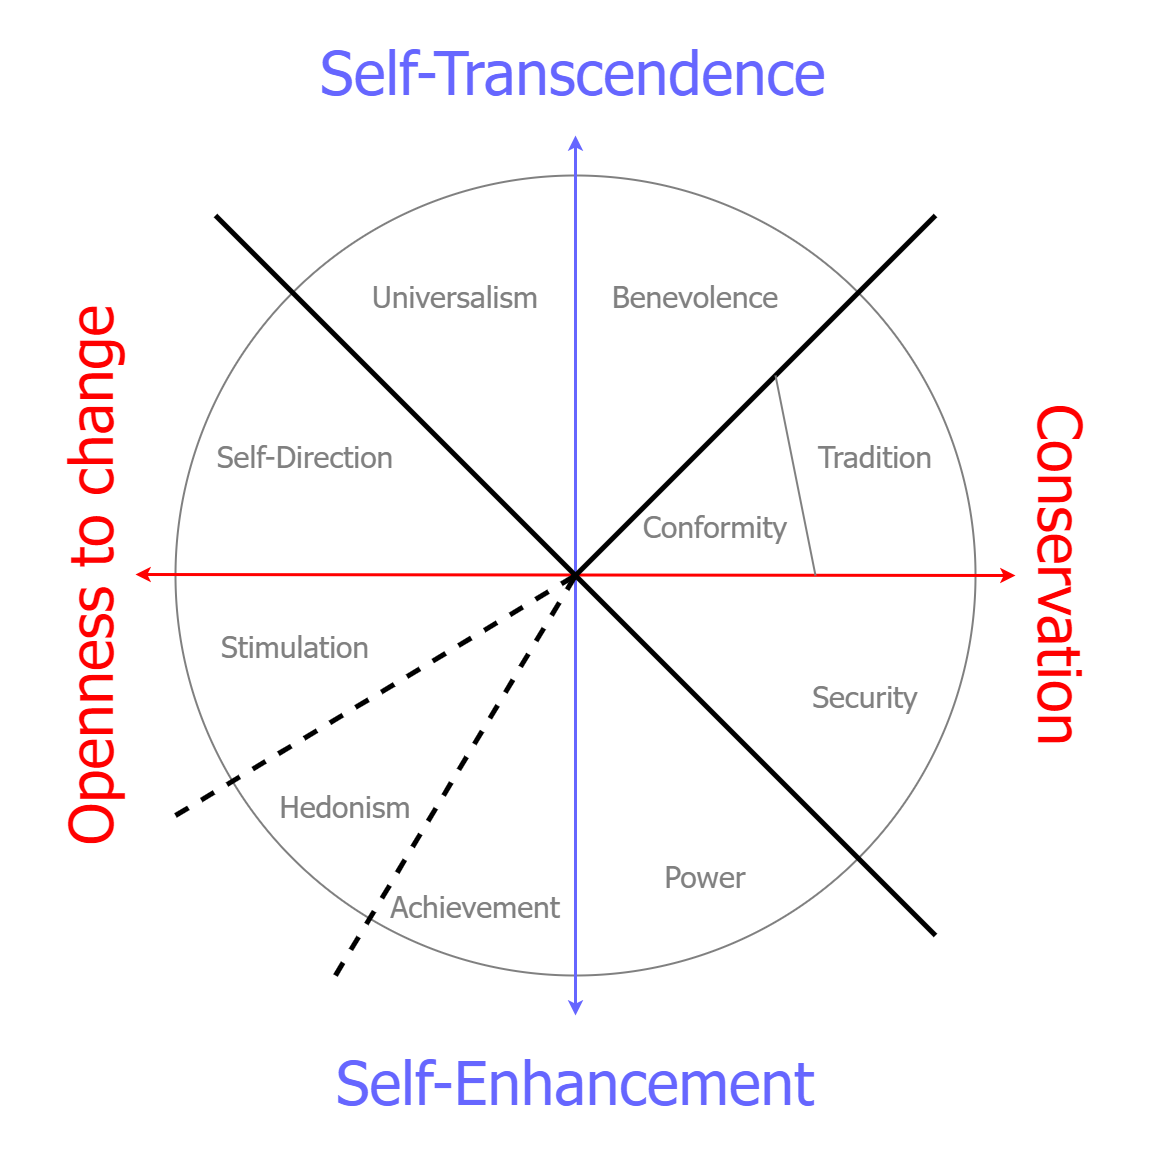
\includegraphics[width=.8\linewidth]{chap3/graphic/schwartz92.png}
	\vspace{-3em}
	\justify\singlespacing\footnotesize{\textit{Notes:} This figure reproduces the two-dimensional structure of motivational types of values from \citet{Schwartz1992Universals, Schwartz2012Overview}.}
\end{figure}